\section{Análisis de Sentimientos}

\subsection{Metodología}

\begin{figure}[H]
    \center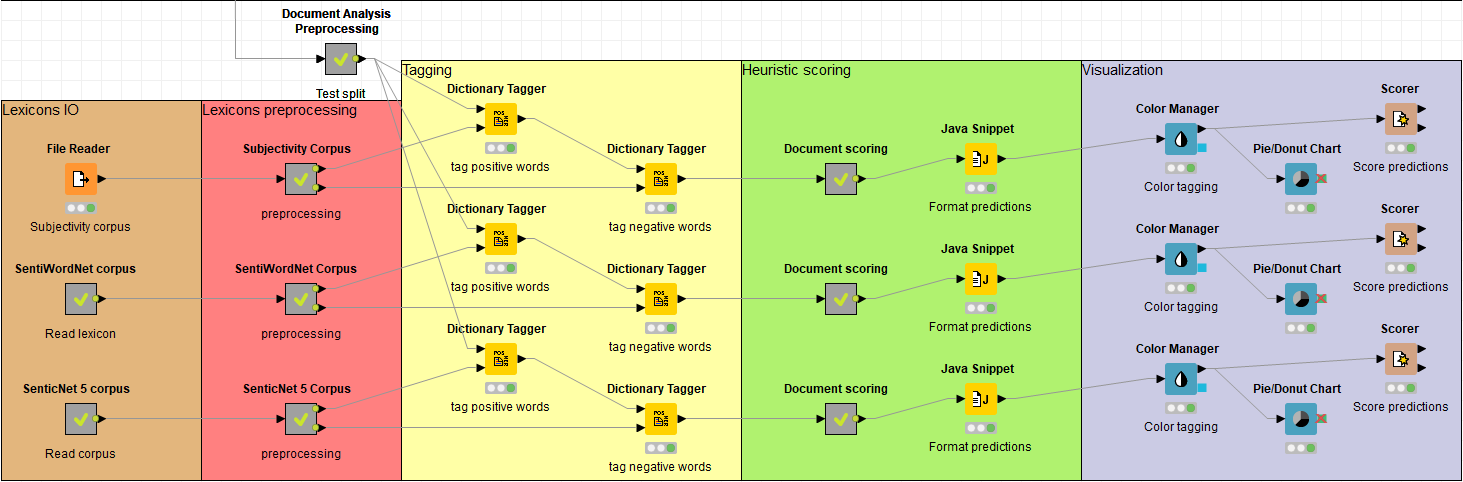
\includegraphics[width=.95\linewidth]{img/analysis/workflow.png}
    \caption{Workflow general del análisis de sentimientos.}
\end{figure}

Para hacer una comparativa justa de resultados, se realiza el análisis de sentimientos sobre la misma partición de test con la que se evalúan los métodos de clasificación.

Como preprocesamiento de los documentos aplicamos un Parts Of Speech tagging y Stanford Lemmatizer para quitar las inflexiones de las palabras.

\vspace{\baselineskip}

Por otro lado, la lectura de los lexicon varía con cada uno:
\begin{itemize}
    \item Para el corpus MPQA se usa el mismo procedimiento proporcionado en clase.
    \item Para SentiWordNet, puesto que cada synsetTerm puede contener más de una palabra, estas se separan en nuevas fila con los mismos valores de sentimiento.

    Seguidamente calculamos el valor de objetividad como $1 - (POS + NEG)$ y a cada término le asignamos un valor \textbf{neutral} si ambos \textit{PosScore} y \textit{NegScore} son iguales, en otro caso se le asigna la etiqueta con el score más alto.

    Por último agrupamos las filas dónde coincidan el synsetTerm, de forma que no se etiqueten algunas palabras con sentimientos diferentes. Para ello hacemos uso del nodo \textit{Group By} y asignamos el sentimiento y el valor de objetividad en base a la moda y a la media respectivamente.
    \item Para SenticNet modificamos el delimitador de columna por uno nuevo, y le asociamos a cada término el valor de \textbf{polarity} proporcionado.
\end{itemize}

\newpage

\begin{figure}[H]
    \center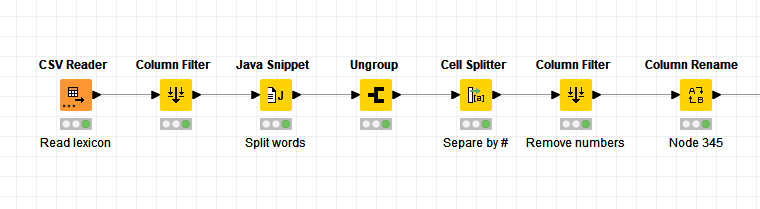
\includegraphics[width=.95\linewidth]{img/analysis/sentiword-reading.png}
    \caption{Lectura del lexicon SentiWordNet.}
\end{figure}

\begin{figure}[H]
    \center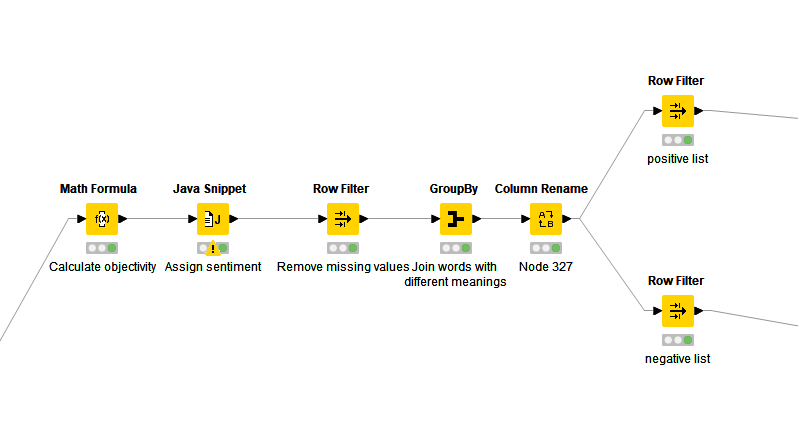
\includegraphics[width=.95\linewidth]{img/analysis/sentiword-prepro.png}
    \caption{Preprocesamiento del lexicon SentiWordNet.}
\end{figure}

\begin{figure}[H]
    \center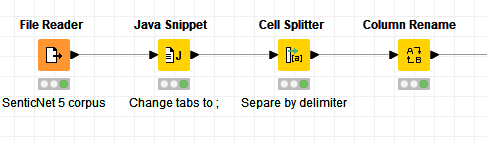
\includegraphics[width=.95\linewidth]{img/analysis/senticnet-reading.png}
    \caption{Lectura del lexicon SenticNet.}
\end{figure}

\newpage

Finalmente para la asignación de sentimiento a cada documento se han usado dos heurísticas diferentes:
\begin{enumerate}
    \item Seleccionado en base al mayor número de palabras que tenga de una etiqueta u otra.
    \item Ponderización según la función del término en la frase (POS), de la siguiente manera: nombres y adjetivos (tanto en singular como en plural) junto a adverbios reciben el doble de peso; conjunciones comparativas (como la cláusula \textit{but}) reciben el triple.
\end{enumerate}

\begin{figure}[H]
    \center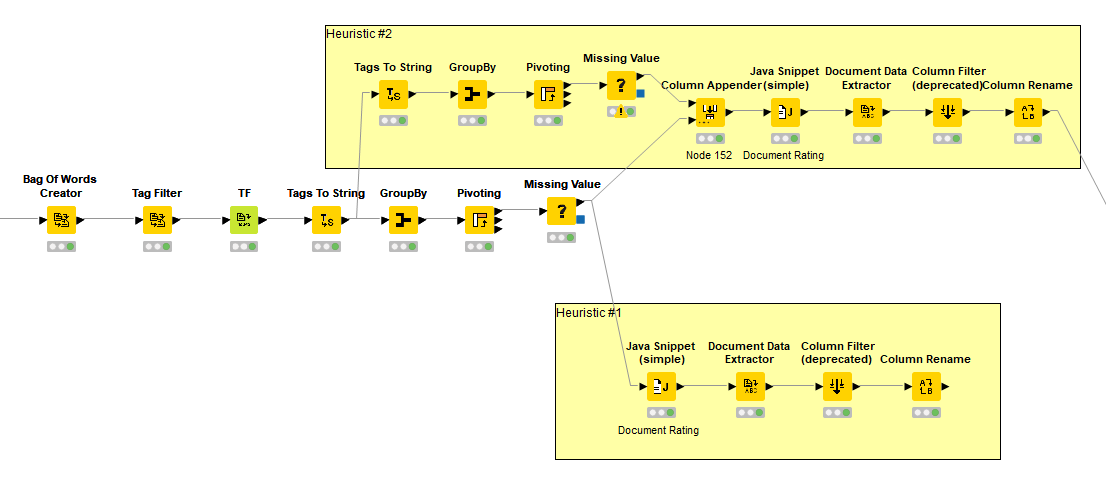
\includegraphics[width=.95\linewidth]{img/analysis/heuristic.png}
    \caption{Cálculo de las diferentes heurísticas. Para la segunda, agrupamos no solo con la etiqueta de sentimiento sino además con la de POS.}
\end{figure}

% -----------

\subsection{Resultados}

\begin{figure}[H]
    \center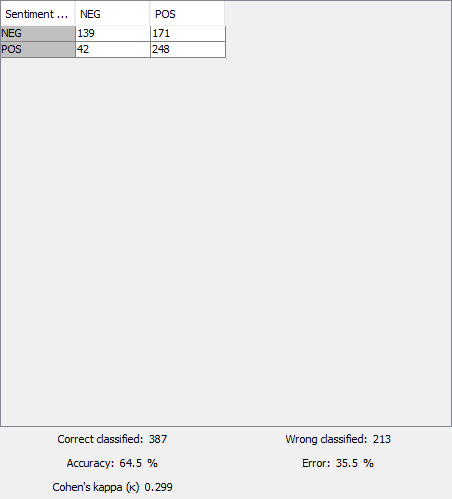
\includegraphics[width=.95\linewidth]{img/analysis/score1.png}
    \caption{Matriz de confusión con MPQA y primera heurística.}
\end{figure}

\begin{figure}[H]
    \center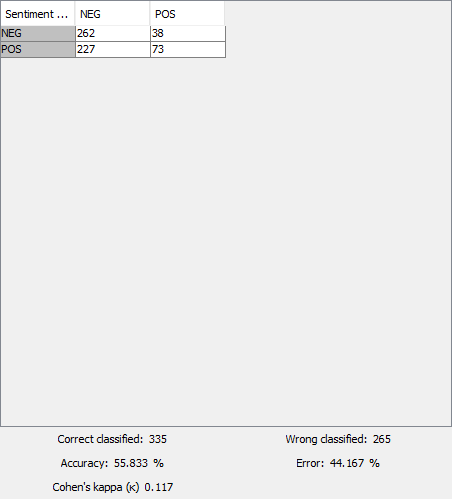
\includegraphics[width=.95\linewidth]{img/analysis/score2.png}
    \caption{Matriz de confusión con SentiWordNet y primera heurística.}
\end{figure}

\begin{figure}[H]
    \center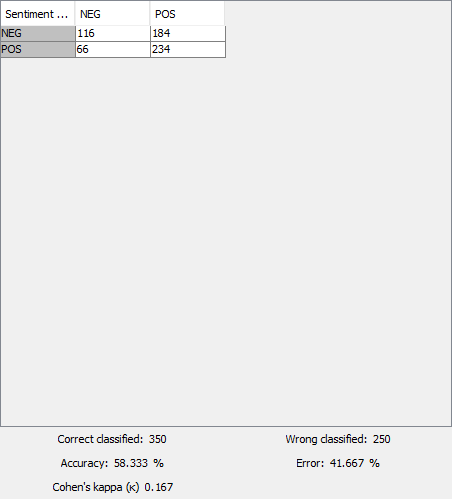
\includegraphics[width=.95\linewidth]{img/analysis/score3.png}
    \caption{Matriz de confusión con SenticNet y primera heurística.}
\end{figure}

\newpage

\begin{figure}[H]
    \center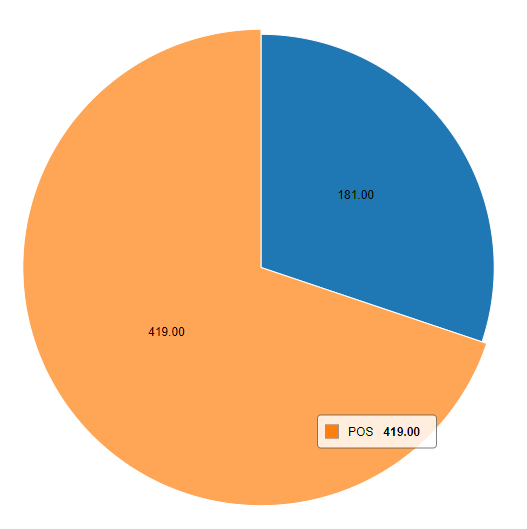
\includegraphics[height=.4\linewidth]{img/analysis/pie1.png}
    \caption{Pie chart con MPQA y primera heurística.}
\end{figure}

\begin{figure}[H]
    \center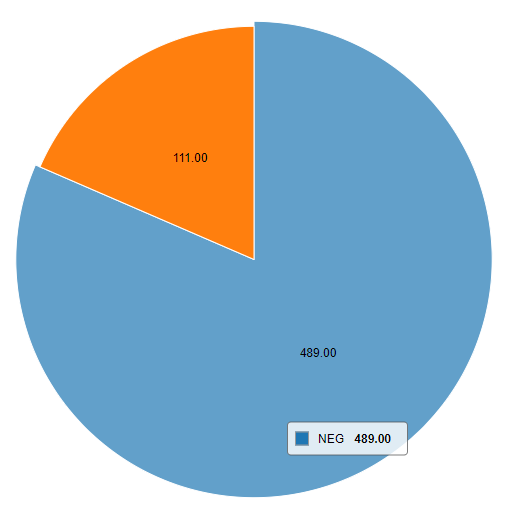
\includegraphics[height=.4\linewidth]{img/analysis/pie2.png}
    \caption{Pie chart con SentiWordNet y primera heurística.}
\end{figure}

\begin{figure}[H]
    \center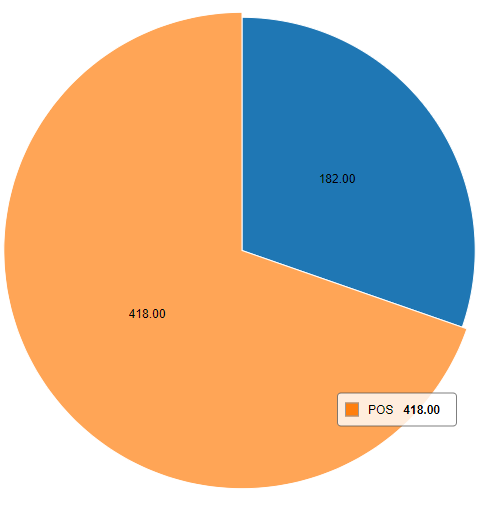
\includegraphics[height=.4\linewidth]{img/analysis/pie3.png}
    \caption{Pie chart con SenticNet y primera heurística.}
\end{figure}

% -------------------

\begin{figure}[H]
    \center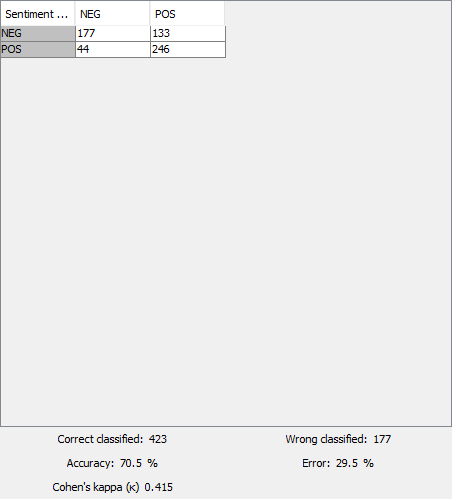
\includegraphics[width=.95\linewidth]{img/analysis/score1-2.png}
    \caption{Matriz de confusión con MPQA y segunda heurística.}
\end{figure}

\begin{figure}[H]
    \center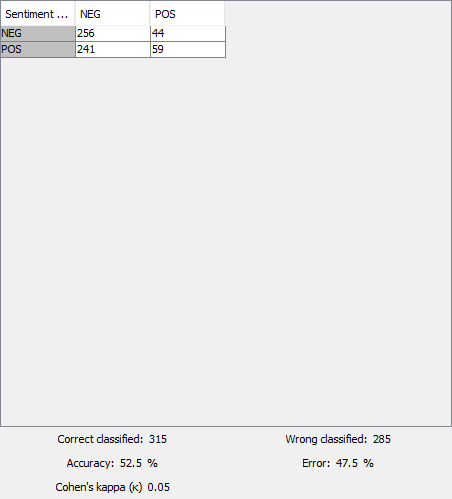
\includegraphics[width=.95\linewidth]{img/analysis/score2-2.png}
    \caption{Matriz de confusión con SentiWordNet y segunda heurística.}
\end{figure}

\begin{figure}[H]
    \center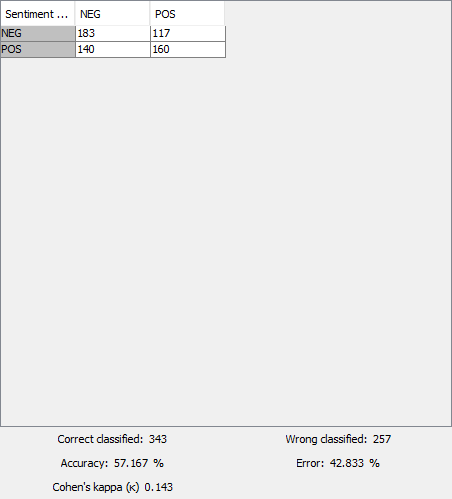
\includegraphics[width=.95\linewidth]{img/analysis/score3-2.png}
    \caption{Matriz de confusión con SenticNet y segunda heurística.}
\end{figure}

\newpage

\begin{figure}[H]
    \center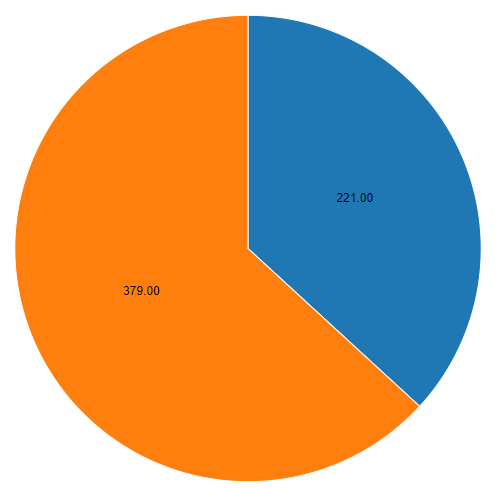
\includegraphics[height=.4\linewidth]{img/analysis/pie1-2.png}
    \caption{Pie chart con MPQA y segunda heurística.}
\end{figure}

\begin{figure}[H]
    \center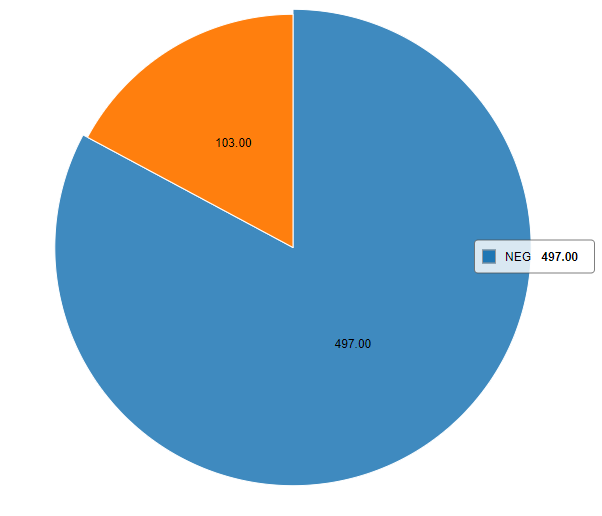
\includegraphics[height=.4\linewidth]{img/analysis/pie2-2.png}
    \caption{Pie chart con SentiWordNet y segunda heurística.}
\end{figure}

\begin{figure}[H]
    \center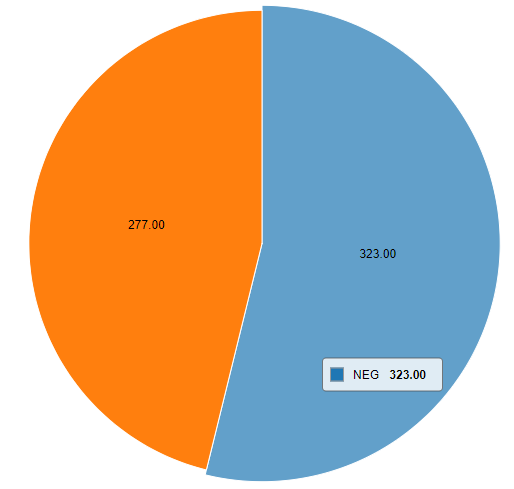
\includegraphics[height=.4\linewidth]{img/analysis/pie3-2.png}
    \caption{Pie chart con SenticNet y segunda heurística.}
\end{figure}